\subsection{Specific Applications}
\label{subsec:03_applications}

In this section we take a closer look at applications that are linked to cybersecurity on a secondary level: Here the Blockchain is not per se used to mitigate direct cybersecurity threats, but is used to make applications more robust, error-prone and less vulnerable. So the Blockchain does solve cybersecurity related issues, but in a more indirect way.

\subsubsection{Assessment Criteria}
Below we want to introduce different scenarios of applications (existing or proof-of-work drafts) for the Blockchain technology and apart from a brief introduction of the challenges and problems of this specific field, answer the following questions:
\begin{enumerate}
	\item What is the quality of this specific type of application regarding cybersecurity? 
	\item How do they make use of the Blockchain Technology?
	\item Is the BC really needed or could the problems be solved without it? 
\end{enumerate}
To answer question number 3 we are going to make use of the below schema presented by \citeauthor{Wust2017} in \cite{Wust2017}, that helps spliting real use cases from unnecessary ones.
\begin{figure}[ht!]
  \begin{center}
  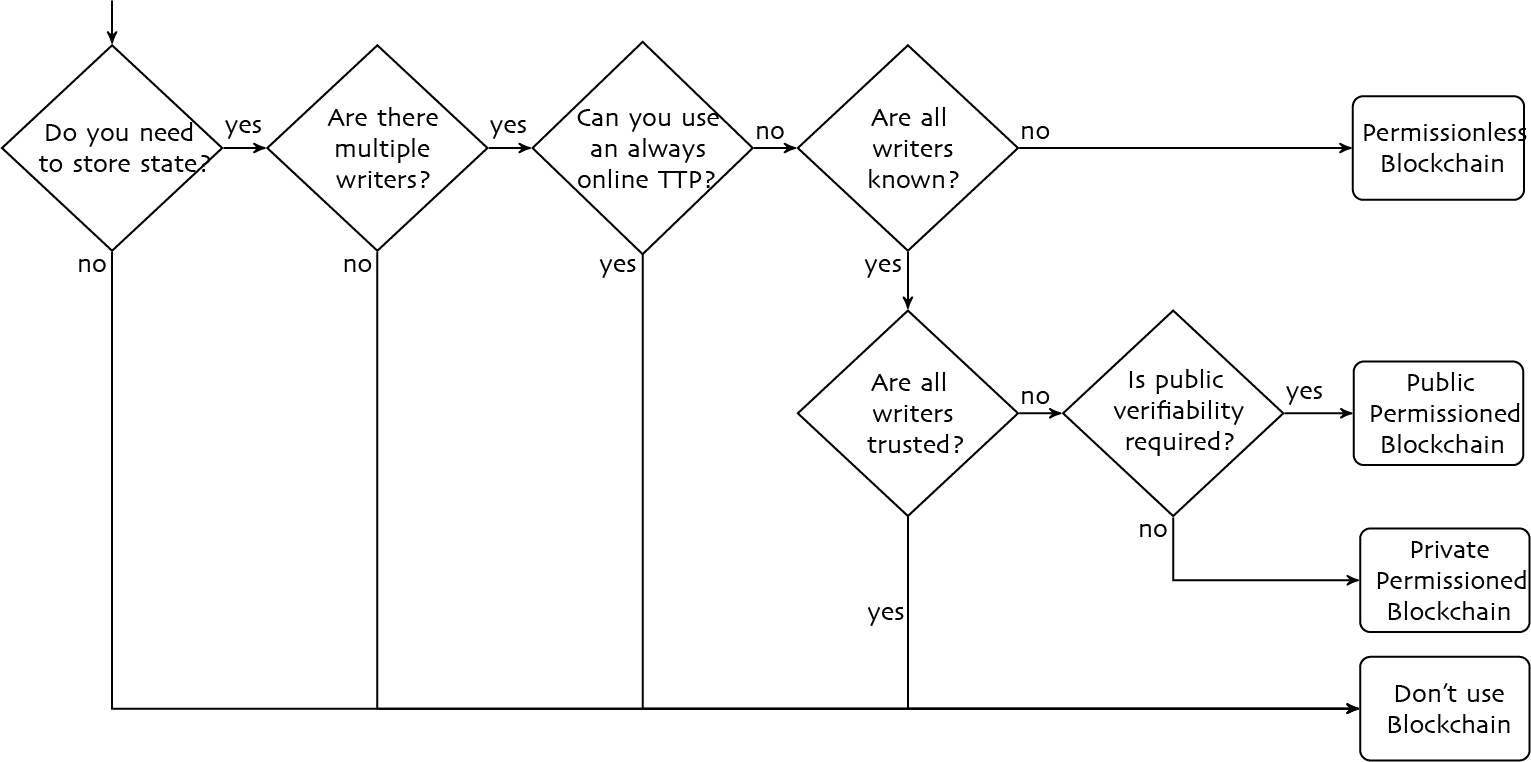
\includegraphics[scale=0.6]{Talk7/img/app/BCorNot}
  \end{center}
  \caption{Do you need a Blockchain?}
  \label{blockchain_or_not}
\end{figure}

\subsubsection{E-Voting}
Problem statement: Foundation of every successful democracy, must be accessible for all eligible citicens. Most common systems today are paper-based voting systems, have two major drawbacks. 1. Not scalable, 2. reliant on the procedural security of officials conducting their jobs. Various combinations exist, multiple security vulnerabilities pop up, that lead to an enourmous risk of election rigging and fraud. The Blockchain as system that is verifiable, scalable and tamper-proof, seems to be a good idea as solution. 

Idea for solution: Use the Blockchain technology for a transparent and incorruptible database that cannot have a single point of failure or be controlled by a single entity. Answers question 1

Several systems exist up till today. Not all rely on the same amount of integration of the Blockchain itself. Different use cases either in theory or in practice have already been tested on smaller county elections or within private organizations \cite{BenAyed2017}.

Estonian I-Voting System: Estonia was the first country where citizens where able to cast their vote online and with an electronic national identification card based on the Blockchain technology
Norwegian I-Voting System: In 2011 Norway used and eletronic remote voting system  for country council elections. The project was 2014 discontinued due to the fear of votes going public in case of a cyber attack.
New South Wales iVote System: In 2015 New South Wales used a hybrid blockchain based voting system.

General problems with the different systems: Single point of failure and closeness of critical parts of the code


Votebook (Quelle): Case study on Blockchain voting. No remote voting due to too many threats. Biggest problems: Authenticating user, voters computer as single point of failure DoS Attack.
Ressembles todays systems, based on paper voting and voting stations that have the Blockchain as backend.
System based on a permissioned, private blockchain with the voting stations as nodes
Follow my Vote (Quelle): Fundamentally different than Votebook. Each voter installs a local "Voting Box" on his computer, authenticating via uploaded official documents through the organization that holds the election. Each voter requests ballot online and votes. Allow for early voting as well as altering the vote later on. Based on  \citeauthor{Osgood2016} optimistic but flawed approach: Authentication and scaring off remote voters is a problem.

Vote Watchers (Quelle): Ressembles Votebook regarding the existence of paper ballots and real world voting stations. Each ballot contains three QR codes - 1 for BC address, 1 for ballot ID, 1 for election ID. Once ballot is scanned, the appropriate vote is sent to proper candidates unique address (like wallet) on an local offline BC of the voting station. After election is complete all data from local blockchain is put on a DVD and the machine is synchronized with the other machines for an evaluation of the voting results. 
Advantage: Offline use, allows no interference from hackers, at the same time the votes for each candidate can be checked in "real time" (??) by a blockchain explorer.
Uses BC only for tamper-proofness and public auditing, with everything else backed on paper ballots.

Proposition of \citeauthor{Osgood2016} is therefore a system that still relies upon paper ballots, where people have to authenticate by showing up in real life at a real world voting booth, that uses the Blockchain for its tamper-proofness and ability to account as an auditing system

Proposition of \citeauthor{BenAyed2017}:
Tries to fulfill the following criteria: 1 (Authentication)Only people already registered to vote can cast votes. The system does not include registration and authentification has to be done externally. 2 (Anonymity) The system will not allow any links between voters votes and identities. 3 (Accuracy) Votes must be accurate and votes can neither be changed, nor duplicated, nor removed. 4 (Verifiablity): The system is verifiable to make sure all votes are counted correctly
Limitations: User as single point of failure is still a problem and inability to change the vote once casted.

General problem: Spotlight too much on the developed part of the world instead of focussing regions where a trust-less system is really used.

Question 3: 
In a voting scenario the authorities need the state of an election to be stored at all times during an election. For one, because of verifiability of the results in the end, but also because of any security related problems that could cause a shutdown of one or multiple of the voting stations. The writers are the voters and need to be known or in any way authenticated by a third party. In this scenario only an organization that has access to all the data is able to do that. In most cases this leaves only the government as a real option. In this scenario the voters per definition do not trust other voters as everyone is assumed to have a different desired output. 
According to the diagram by  \citeauthor{Wust2017} the use of Blockchain technology therefore only makes sense in country where the government is not a thrusted third party. In which case a public permissioned Blockchain would be the best solution.
Nevertheless, it is the role of the government that causes the dilemma itself. If the non-existing trust in the government is the justification for the use of the Blockchain, the question arises whether the government can be trusted regarding the authentication of the voters. Even though a systematic rigging is harder to achieve with this approach, the problem remains at hand. 

While the Blockchain does seem to be perfect for a voting situations, its justification remains questionable. Especially, because it still leaves the most important point of failure unprotected: The user himself. Even the most tamperproofed, blockchain-based voting system does not prevent hackers from a man-in-the-middle attack from a compromised end-device. 

To sum this chapter up: Many of the desired e-Voting properties that the Blockchain technology provides have trade-offs. The aspect of privacy is just one of many. On the other hand, no system has yet been proposed that has been shown to be secure, verifiable and private at the same time. The question of authentifiation comes into play as additional point of failure of the concept.
Therefore: If a online trusted third party exists, the use of the blockchain is not necessary. If the government is trusted as far as the authentification of the voters goes, a public permissioned Blockchain can be a good fit. However the security of the system then relies on the interity of the validators. 
If the government is trusted not at all, there exists no solution that overcomes that systematic flaw in a countries governance.

The Blockchain can therefore be a solution if the question of authentification can be answered satisfactorily. Otherwise a traditional paper based voting system is as good as voting system including Blockchain based systems or systems that base on a trusted third party.

\subsubsection{Autonomous Vehicles}
\begin{itemize}
	\item \cite{Dorri2017}
	\item  \cite{Rowan2017}
	\item \cite{Sharma2017}
\end{itemize}
\subsubsection{Personal Data Protection and Patient Monitoring}
\begin{itemize}
	\item \cite{Zyskind2015}
	\item \cite{Yue2016}
	\item \cite{Azaria2016}
	\item \cite{Fotiou2016}
	\item \cite{Zhang2017}
	\item \cite{Zhang2018}
	\item \cite{Esposito2018}
	\item \cite{Ekblaw2016}
	\item \cite{Cao2019}
\end{itemize}
\subsubsection{Smart Cities \& IoT}
\begin{itemize}
	\item \cite{Biswas2016}
	\item \cite{Mylrea2017}
	\item \cite{Liang2018}
	\item \cite{Dorri2017a}
	\item \cite{Shafagh2017}
\end{itemize}

